\documentclass[12pt, a4paper]{article}
\usepackage{graphicx}
\usepackage{xurl}
\usepackage{geometry}
\usepackage{float}
\usepackage{indentfirst}
\geometry{left=2.54cm, right=2.54cm, top=3.18cm, bottom=3.18cm}
% \setlength{\parindent}{0pt}

\title{Weekly Report}
\author{Jerry Jin}

\begin{document}

\maketitle

\section*{Week 01/08}

\subsection*{Rethink on the Feedforward Network}

% Last week, I demonstrated a way to transfer learning in gains and shifts to weights. However, it is based on switching hebbian learning on and off frequently: only if the loss for a particular data point is small, hebbian learning is performed. I also actively narrow the gains and shifts boundary. It turns out that it does not work well for RNN or adpatation to perturbation.

Ideally, after doing backprop on gains and shifts, the response tuning curves of side neurons would go up and those of middle neurons would go down. Then, when hebbian learning is turning on, the weights of side neurons would get larger update than those of middle nuerons, resulting in a cosine-like weights. The next rounds of backprop would flatten the response tuning curves to maintain a low loss. In theory, this process transfers the learning in gains and shifts to weights. (We don't really need the active shrinkage of gains and shifts. In fact, if the shrinkage/flattening goes too fast, hebbian learning could not result in enough curvature in weights.)

In practice, the process could not transfer the learning completely, returning the gains and shifts to the initial values. It would converge to a state where the learning is partly in weights and partly in gains and shifts. 

\begin{figure}[H]
    \centering
    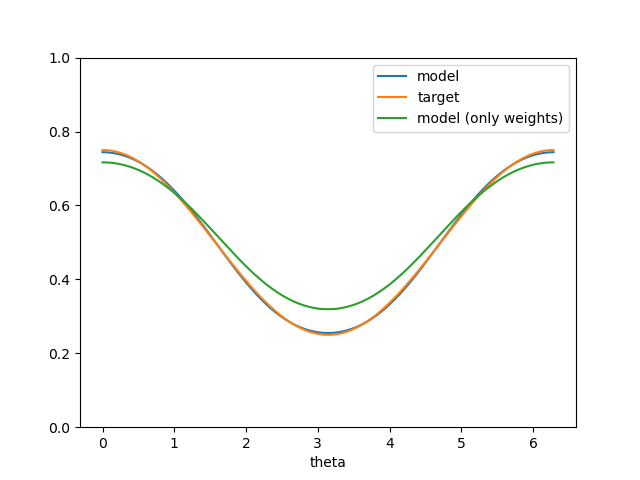
\includegraphics[width=0.3\textwidth]{baseline_abb05/fig/0122_abb05_bphebb_onlyweights.png}
    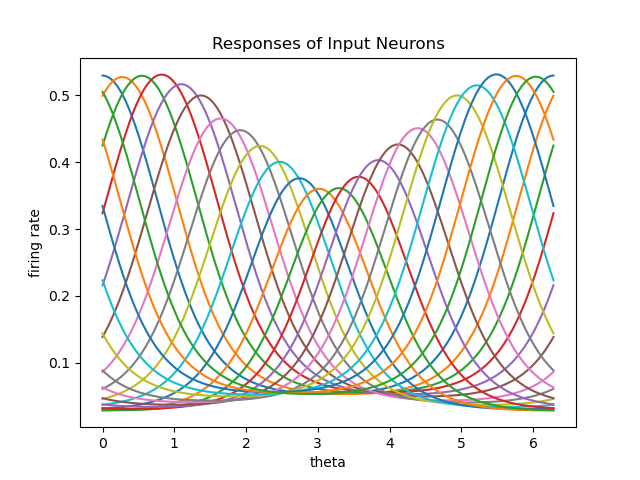
\includegraphics[width=0.3\textwidth]{baseline_abb05/fig/0122_abb05_bphebb_rf.png}
    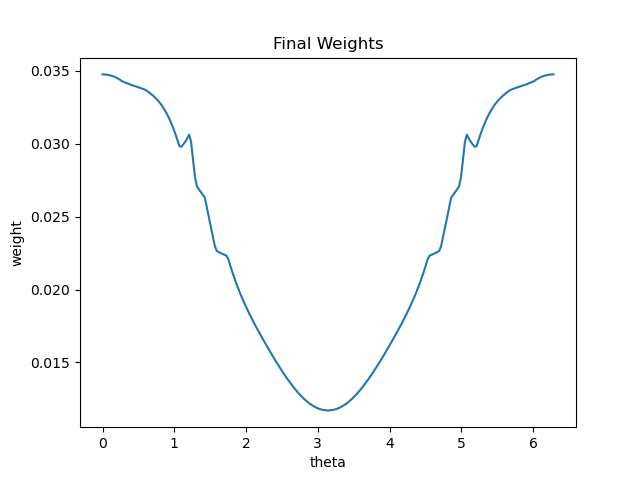
\includegraphics[width=0.3\textwidth]{baseline_abb05/fig/0122_abb05_bphebb_weights.png}
    \\
    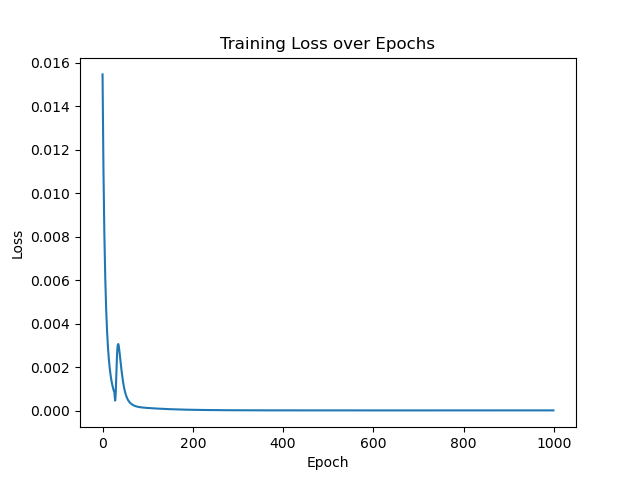
\includegraphics[width=0.3\textwidth]{baseline_abb05/fig/0122_abb05_bphebb_loss.png}
    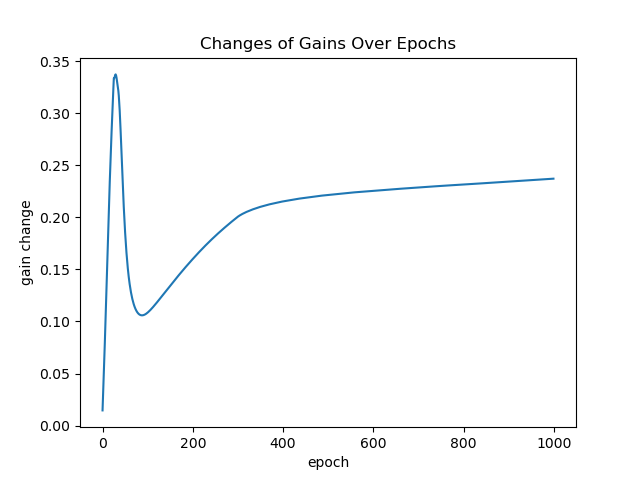
\includegraphics[width=0.3\textwidth]{baseline_abb05/fig/0122_abb05_bphebb_gc.png}
    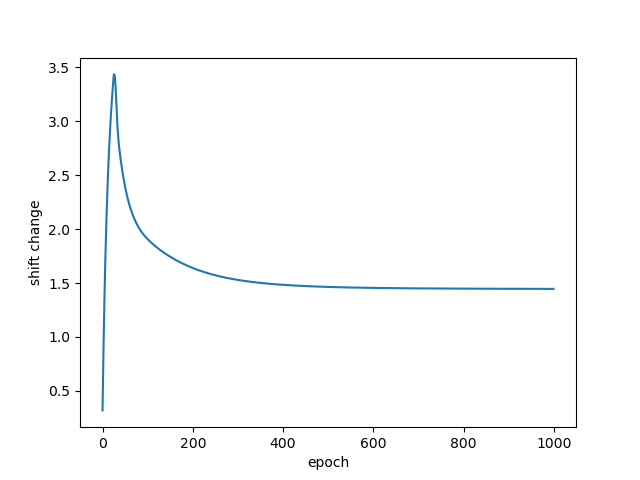
\includegraphics[width=0.3\textwidth]{baseline_abb05/fig/0122_abb05_bphebb_sc.png}\\
    \caption{Hebbian learning start after 10 epoches.}
    \label{fig:1}
\end{figure}

To understand this, I did an experiment where I keep the gains and shifts unchanged as initial and use backprop to find the "correct" weights. Then I turn on the hebbian learning, but the "correct" weights is not stable. In fact, it would converge to some weights whose loss is high. In other words, the "correct" weights is not a convergence point of hebbian learning.

% fig

Mathemetically, the "correct" weights should meet some requirements to be the convergence point of hebbian learning.


\newpage

\subsection*{Transfer of learning in RNN}

I implement the same training paradigm to train the RNN, i.e., first do backprop on gains and shifts and then turn on hebbian learning, to see how much of the learning could be transfered from gains and shifts to weights.

Some details: 16 nodes in recurrent layer; hebbian learning is done for every timestep; evenly distributed gaussian receptive fields for each neuron; output weight matrix are set to all 1s.

For inhibitory synaptic plasticity, I didn't find a principle for firing rate. Existing attempts are all based on spike timings. So I just use the same idea as in excitatory synapses: the more they are firing together, the inhibitory synapses are stronger (more negative).

\begin{figure}[H]
    \centering
    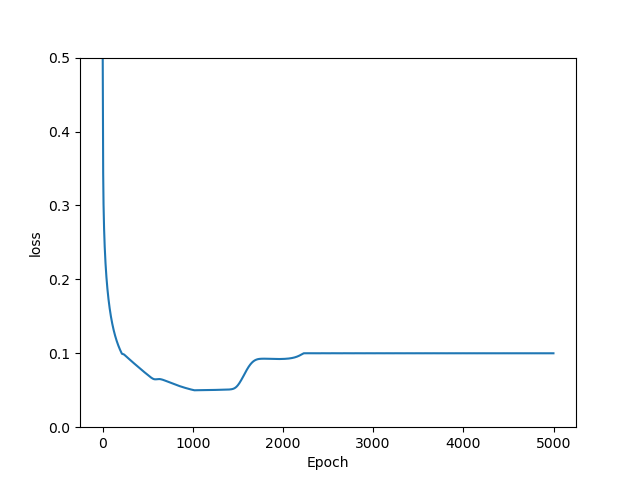
\includegraphics[width=0.45\textwidth]{fig/sin_gn_loss.png} \\
    \label{fig:1}
\end{figure}

123123123

\newpage

\end{document}